\documentclass[12pt, a4paper]{article}

% ==========================================
% 1. KHAI BÁO GÓI THƯ VIỆN (PACKAGES)
% ==========================================
% Bảng mã & Font chữ
\usepackage[utf8]{inputenc}
\usepackage[T5]{fontenc}

% Toán học
\usepackage{amsmath, amssymb}

% Căn lề & Bố cục trang
\usepackage[top=2.2cm, bottom=1.5cm, left=1cm, right=1cm, headheight=15pt]{geometry}
\usepackage{fancyhdr}
\usepackage{needspace}
\usepackage{tkz-tab}

% Đồ họa & Màu sắc
\usepackage{xcolor}
\usepackage{graphicx} 
\usepackage{tikz}
\usetikzlibrary{calc, shapes.geometric, positioning}


% Bảng biểu & Danh sách
\usepackage{colortbl}
\usepackage{array}
\usepackage{makecell}
\usepackage{multirow}
\usepackage{tasks}

% Biểu tượng
\usepackage{fontawesome5}

% ==========================================
% 2. THIẾT LẬP MÀU SẮC CHỦ ĐẠO
% ==========================================
\definecolor{goldyellow}{RGB}{255, 179, 0}
\definecolor{amberorange}{RGB}{230, 115, 0}
\definecolor{lightamber}{RGB}{255, 248, 225}
\definecolor{deepblue}{RGB}{25, 42, 86}
\definecolor{accentred}{RGB}{232, 65, 24}
\definecolor{softgray}{RGB}{220, 220, 222} 
\definecolor{fbblue}{RGB}{15, 80, 200}


% ==========================================
% 3. CẤU HÌNH HEADER & FOOTER
% ==========================================
\pagestyle{fancy}
\fancyhf{}
\renewcommand{\headrulewidth}{0pt}

% Khai báo biến lưu trữ nội dung góc phải của Header
\newcommand{\HeaderRightText}{}

% --- Header ---
\fancyhead[C]{
    \begin{tikzpicture}[remember picture, overlay]
        
        % Dải màu trang trí góc trên
        \path[fill=deepblue] (current page.north west) -- (current page.north east) 
            -- ($(current page.north east) + (0, -1.6cm)$) 
            .. controls ($(current page.north) + (3, -2.0cm)$) and ($(current page.north) + (-3, -0.4cm)$) .. 
            ($(current page.north west) + (0, -1.0cm)$) -- cycle;
            
        \path[fill=goldyellow] (current page.north west) -- (current page.north east) 
            -- ($(current page.north east) + (0, -1.0cm)$) 
            .. controls ($(current page.north) + (4, -1.0cm)$) and ($(current page.north) + (-2, -2.2cm)$) .. 
            ($(current page.north west) + (0, -1.6cm)$) -- cycle;
            
        \path[fill=amberorange] (current page.north west) -- ($(current page.north west) + (6.5cm, 0)$) 
            .. controls ($(current page.north west) + (4.5cm, -1.2cm)$) and ($(current page.north west) + (2cm, -2.0cm)$) .. 
            ($(current page.north west) + (0, -2.0cm)$) -- cycle;
            
        % Logo góc trái Header
        \node[anchor=west, inner sep=0pt] 
            at ($(current page.north west) + (0cm, -0.8cm)$) {
\includegraphics[height=2.0cm]{../../../image/logo-header.png}};
            
        % Text góc phải Header (Tự động lấy từ đối số thứ 3 của \titlebox)
        \node[anchor=east, text=white, font=\small\bfseries\sffamily] 
            at ($(current page.north east) + (-0.8cm, -0.5cm)$) {\HeaderRightText};
    \end{tikzpicture}
}

% --- Footer ---
\fancyfoot[C]{
    \begin{tikzpicture}[remember picture, overlay]
        % Đường kẻ ngang
        \draw[amberorange, line width=1.5pt] 
            ($(current page.south west) + (0cm, 0.4cm)$) -- ($(current page.south east) + (0cm, 0.4cm)$);

        % Dải cong góc phải
        \path[fill=goldyellow] (current page.south east) -- ($(current page.south east) + (-5cm, 0)$) 
            .. controls ($(current page.south east) + (-3cm, 0.8cm)$) and ($(current page.south east) + (-1.5cm, 1.2cm)$) .. 
            ($(current page.south east) + (0, 1.2cm)$) -- cycle;

        % Mạng xã hội
        \node[anchor=west, inner sep=0pt] at ($(current page.south west) + (1cm, 0.8cm)$) {
            \small\sffamily
            \textcolor{fbblue}{\faFacebook\hskip 4pt Toán Anh Huy MATH-STER}
            \hskip 18pt
            \textcolor{black}{\faTiktok\hskip 4pt huymathster}
        };

        % Số trang
        \node[circle, fill=white, draw=amberorange, line width=1.5pt, text=deepblue, font=\large\bfseries\sffamily, inner sep=4pt, minimum size=0.8cm] 
            at ($(current page.south east) + (-1.2cm, 0.6cm)$) {\thepage};
    \end{tikzpicture}
}

% ==========================================
% 4. ĐỊNH NGHĨA MACRO: KHUNG TIÊU ĐỀ
% ==========================================
\newcommand{\titlebox}[3]{
    % Gán nội dung đối số #3 vào biến HeaderRightText
    \gdef\HeaderRightText{#3}
    
    \begin{center}
    \vspace*{-0.5cm}
    \begin{tikzpicture}
        % Khung vô hình (Phantom Box) định chuẩn kích thước
        \node[text width=16cm, inner xsep=0pt, inner ysep=16pt, opacity=0] (MainBox) {
            \begin{minipage}[c]{4.2cm}
                \centering\vspace{0.1cm}
                \rule{2.2cm}{2.2cm} 
                \vspace{0.1cm}
            \end{minipage}%
            \begin{minipage}[c]{11.5cm}
                \centering\vspace{0.15cm}
                {\huge\bfseries\sffamily #2 \par}
                \vspace{0.15cm} 
            \end{minipage}
        };
        
        % Đổ bóng & Nền
        \fill[goldyellow, rounded corners=8pt] ([xshift=5pt, yshift=-5pt]MainBox.south west) rectangle ([xshift=5pt, yshift=-5pt]MainBox.north east);
        \fill[white, rounded corners=8pt] (MainBox.south west) rectangle (MainBox.north east);
        
        % Lưới ô ly & Nền Logo
        \begin{scope}
            \clip[rounded corners=8pt] (MainBox.south west) rectangle (MainBox.north east);
            \draw[step=0.4cm, softgray!50, line width=0.6pt] (MainBox.south west) grid (MainBox.north east);
            \fill[lightamber!60] (MainBox.south west) rectangle ([xshift=4.2cm]MainBox.north west);
        \end{scope}

        % Viền ngoài
        \draw[deepblue, line width=1.5pt, rounded corners=8pt] (MainBox.south west) rectangle (MainBox.north east);

        % Nội dung Text (Lớp trên cùng)
        \node[text width=16cm, inner xsep=0pt, inner ysep=16pt] at (MainBox.center) {
            \begin{minipage}[c]{4.2cm}
                \centering
                % --- ĐIỀU CHỈNH TỌA ĐỘ LOGO Ở ĐÂY ---
                \hspace*{-0.5cm}\raisebox{-0.2cm}{
\includegraphics[width=5.5cm]{../../../image/logo.png}}
            \end{minipage}%
            \begin{minipage}[c]{11.5cm}
                \centering\vspace{0.15cm}
                {\huge\bfseries\sffamily\color{deepblue} #2 \par}
                \vspace{0.15cm} 
            \end{minipage}
        };
        
        % Trang trí phụ kiện
        \draw[deepblue, line width=1.5pt, dashed] ([xshift=4.2cm]MainBox.north west) -- ([xshift=4.2cm]MainBox.south west);
        \node[regular polygon, regular polygon sides=4, rotate=45, fill=white, draw=accentred, line width=1.2pt, inner sep=2.5pt] at ([xshift=4.2cm]MainBox.west) {};
        \node[anchor=west, fill=amberorange, text=white, font=\large\bfseries\sffamily, rounded corners=4pt, draw=deepblue, line width=1.5pt, inner xsep=12pt, inner ysep=6pt] at ([xshift=1.5cm]MainBox.north west) {#1};
        \fill[accentred] ([xshift=-1.8cm, yshift=-0.4cm]MainBox.north east) circle (3pt);
        \fill[amberorange] ([xshift=-1.4cm, yshift=-0.4cm]MainBox.north east) circle (3pt);
        \fill[goldyellow] ([xshift=-1.0cm, yshift=-0.4cm]MainBox.north east) circle (3pt);
    \end{tikzpicture}
    \vspace*{0cm}
    \end{center}
}

% ==========================================
% 5. ĐỊNH NGHĨA MACRO: CẤU TRÚC CÂU HỎI (ÉP SÁT NHAU)
% ==========================================
\newcommand{\questioncore}[2]{
    % Xóa khoảng cách phía trên, ép sát câu trước
    \noindent \textbf{\textcolor{deepblue}{Câu #1.} \textcolor{accentred}{[STER]}} #2
    \par\nopagebreak
}

% Cấu hình hiển thị đáp án trắc nghiệm
\settasks{
    label=\textbf{\textcolor{amberorange}{\Alph*.}}, 
    label-width=15pt,     
    item-indent=25pt,     
    label-offset=6pt,    
    column-sep=20pt,     
    after-item-skip=2pt  % Đã giảm tối đa khoảng cách giữa các dòng đáp án A B C D
}

% Hàm vẽ dòng kẻ nháp
\newcommand{\drawdashlines}[1]{
    \ifnum#1>0
        \nopagebreak\vspace{0.1cm}\noindent 
        \begin{tikzpicture}
            \foreach \i in {1,...,#1} {
                \draw[softgray, line width=0.2pt] (0,-{\i*1}) -- (\textwidth-4pt,-{\i*1});
            }
        \end{tikzpicture}
        \par
    \fi
    % Đã xóa hoàn toàn khoảng cách thừa ở nhánh else
}

% --- Dạng 1: Trắc nghiệm 4 đáp án ---
\newcommand{\questionLinesManual}[4]{
    \pgfmathsetmacro{\calculatedSpace}{1.5 + #1 * 0.65}
    \needspace{\calculatedSpace cm} 
    \questioncore{#2}{#3}
    #4
    \par\nopagebreak
    \drawdashlines{#1}
}


% --- Dạng 2: Trắc nghiệm Đúng/Sai ---
\newcommand{\questionTrueFalse}[4]{
    \scriptsize
    \pgfmathsetmacro{\calculatedSpace}{3.0 + #1 * 0.65} 
    \needspace{\calculatedSpace cm}
    \questioncore{{#2}}{#3}
    
    \nopagebreak
    \begin{flushleft}
    \renewcommand{\arraystretch}{1.2} % Bóp nhỏ chiều cao của bảng Đ/S
    \begin{tabular}{|>{\centering\arraybackslash}m{0.4cm}|m{6cm}|>{\centering\arraybackslash}m{1cm}|>{\centering\arraybackslash}m{1cm}|}
        \hline
        \rowcolor{amberorange!20}
        & \multicolumn{1}{>{\centering\arraybackslash}m{6cm}|}{\textbf{\textcolor{deepblue}{Mệnh đề}}} & 
        \textbf{\textcolor{deepblue}{Đúng}} & 
        \textbf{\textcolor{deepblue}{Sai}} \\
        \hline
        #4
        \hline
    \end{tabular}
    \renewcommand{\arraystretch}{1}
    \end{flushleft}
    
    \par\nopagebreak
    \drawdashlines{#1}
}

% ----- Dạng 3: Tự luận ngắn -----
\newcommand{\questionShortAnswer}[3]{
    \scriptsize
    \pgfmathsetmacro{\calculatedSpace}{1.5 + #1 * 0.8}
    \needspace{\calculatedSpace cm}
    
    {\linespread{1.1}\selectfont % Bóp nhỏ giãn dòng của câu tự luận
    \questioncore{#2}{#3}\par}
    
    \nopagebreak
    \begin{flushright}
        \begin{tikzpicture}
            \node[anchor=east, font=\small\bfseries\sffamily, text=deepblue] 
                at (-0.2, 0.4) {Đáp án:};
            \fill[goldyellow, rounded corners=3pt] (0.08, -0.08) rectangle (3.08, 0.72);
            \draw[draw=deepblue, fill=white, line width=1.2pt, rounded corners=3pt] 
                (0,0) rectangle (3.0, 0.8);
            \foreach \x in {0.75, 1.5, 2.25} {
                \draw[draw=deepblue, line width=0.6pt] (\x, 0) -- (\x, 0.8);
            }
        \end{tikzpicture}
    \end{flushright}
    
    \par\nopagebreak
    \drawdashlines{#1}
}

% ==========================================
% BẮT ĐẦU NỘI DUNG TÀI LIỆU
% ==========================================
\begin{document}

% Truyền 3 tham số: {Nhãn cam} {Chữ to chính giữa} {Chữ ở góc phải Header}
\titlebox{Chủ đề: Hàm số}{Ứng dụng khảo sát đồ thị hàm số}{Hàm số: Ứng dụng đồ thị}

\drawdashlines{20}
\newpage
\drawdashlines{25}
\newpage

% --- CÂU 9 ---
\questionShortAnswer{15}{1}{Một phần đường chạy của tàu lượn siêu tốc (hình 1) khi gắn hệ trục tọa độ Oxy được mô phỏng ở hình 2, đơn vị trên mỗi trục là mét. Biết đường chạy của nó là một phần đồ thị hàm bậc ba  
\(y = ax^3 + bx^2 + cx + d \quad (0 \leq x \leq 90)\)
; tàu lượn siêu tốc xuất phát từ điểm \( A \), đi qua các điểm \( C, D \) đồng thời đạt độ cao nhỏ nhất so với mặt đất là \( 6m \). Độ cao lớn nhất mà tàu lượn siêu tốc đạt được là bao nhiêu mét so với mặt đất (kết quả làm tròn đến hàng phần chục)?
\begin{figure}[h!]
    \centering
    % --- HÌNH 1 (BÊN TRÁI): ẢNH CHÈN VÀO ---
    \begin{minipage}[b]{0.4\textwidth}
        \centering
        % Thay "rollercoaster.png" bằng tên file ảnh của bạn
        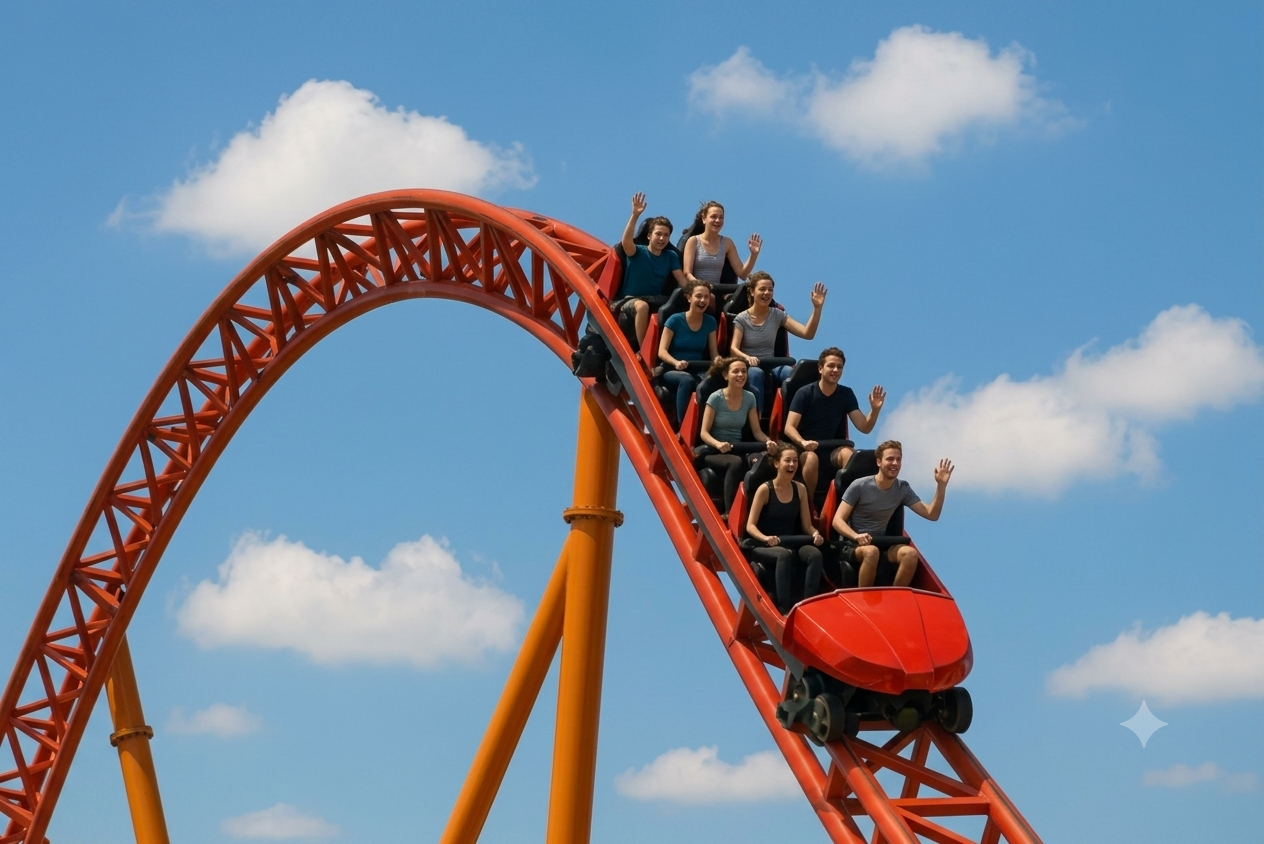
\includegraphics[width=\textwidth]{../images/TauLuon.png}
        \par\vspace{1.5ex} % Tạo khoảng cách nhỏ giữa hình và chữ
        \textbf{Hình 1}
    \end{minipage}
    \hfill
    % --- HÌNH 2 (BÊN PHẢI): ĐỒ THỊ TIKZ ---
    \begin{minipage}[b]{0.4\textwidth}
        \centering
        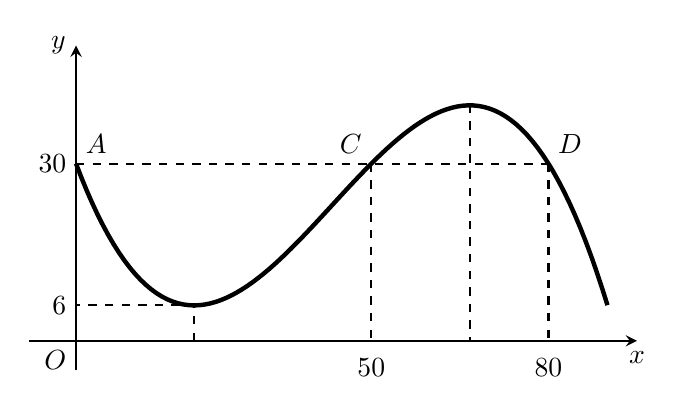
\begin{tikzpicture}[>=stealth, scale=0.75]
            % Vẽ hệ trục tọa độ Oxy
            \draw[->, thick] (-0.8, 0) -- (9.5, 0) node[below] {$x$};
            \draw[->, thick] (0, -0.5) -- (0, 5.0) node[left] {$y$};
            \node[below left] at (0,0) {$O$};

            % Vẽ đường cong đồ thị
            \draw[ultra thick, samples=100, domain=0:9.0] 
                plot (\x, {-1/15*\x^3 + 13/15*\x^2 - 8/3*\x + 3});

            % Đường nét đứt gióng từ các điểm quan trọng
            \draw[dashed, thick] (2, 0) -- (2, 0.6) -- (0, 0.6);
            \draw[dashed, thick] (0, 3) -- (8, 3);
            \draw[dashed, thick] (5, 3) -- (5, 0);
            \draw[dashed, thick] (6.67, 4) -- (6.67, 0);
            \draw[dashed, thick] (8, 3) -- (8, 0);

            % Các nhãn điểm trên đồ thị
            \node[above right] at (0, 3) {$A$};
            \node[above left] at (5, 3) {$C$};
            \node[above right] at (8, 3) {$D$};

            % Các nhãn số trên trục tọa độ
            \node[left] at (0, 3) {$30$};
            \node[left] at (0, 0.6) {$6$};
            \node[below=3pt] at (5, 0) {$50$};
            \node[below=3pt] at (8, 0) {$80$};
        \end{tikzpicture}
        \par\vspace{1.5ex} % Tạo khoảng cách nhỏ giữa hình và chữ
        \textbf{Hình 2}
    \end{minipage}
\end{figure}}


% --- CÂU 11 ---
\questionShortAnswer{15}{2}{Một hồ nước nhân tạo được xây dựng trong công viên giải trí. Trong mô hình minh họa sau, nó được giới hạn bởi các trục tọa độ và đồ thị hàm số \( y = f(x) = -x^3 + 5x^2 - \dfrac{21}{2}x + 10 \). Đơn vị đo độ dài trên mỗi trục tọa độ là \( 100m \). Trong công viên có một con đường chạy dọc theo đồ thị của hàm số \( y = -\dfrac{7}{2}x + 24 \). Người ta dự định xây dựng bên bờ hồ một bến thuyền đạp nước sao cho khoảng cách từ bến thuyền đến con đường là ngắn nhất. Khi đó tọa độ của điểm để xây bến thuyền là \( M(a; b) \). Tính \( T = 3a - 54b \).

\begin{center}
\begin{tikzpicture}[>=stealth, scale=0.5]

    % =================================================================
    % 1. VẼ PHẦN TÔ MÀU DIỆN TÍCH "HỒ NƯỚC" (HÌNH PHẲNG GIỚI HẠN)
    % =================================================================
    % Đồ thị f(x) cắt trục hoành tại x = 2 (vì f(2) = -8 + 20 - 21 + 10 = 1)
    % Để phần tô màu khớp hoàn toàn với đồ thị, ta dùng cấu trúc fill với hàm số
    \fill[gray!40] (0,0) -- (0,10) 
        plot[domain=0:2.35, samples=100] (\x, {-\x^3 + 5*\x^2 - 10.5*\x + 10}) 
        -- (0,0) -- cycle;

    % Chữ "hồ nước" đặt bên trong vùng tô màu
    \node[align=center, scale=0.8] at (0.7, 1.2) {hồ\\nước};

    % =================================================================
    % 2. VẼ HỆ TRỤC TỌA ĐỘ Oxy
    % =================================================================
    \draw[->, thick] (-1.0, 0) -- (9.0, 0) node[below] {$x$};
    \draw[->, thick] (0, -1.5) -- (0, 11.5) node[left] {$y$};
    \node[below left] at (0,0) {$O$};

    % Vạch chia và số trên trục hoành (Ox)
    \foreach \x in {2, 4, 6, 8} {
        \draw[shift={(\x,0)}, thin] (0pt,2pt) -- (0pt,-2pt) node[below] {$\x$};
    }

    % Vạch chia và số trên trục tung (Oy)
    \foreach \y in {2, 4, 6, 8} {
        \draw[shift={(0,\y)}, thin] (2pt,0pt) -- (-2pt,0pt) node[left] {$\y$};
    }

    % =================================================================
    % 3. VẼ ĐỒ THỊ CÁC HÀM SỐ
    % =================================================================
    % Đồ thị hàm số y = f(x)
    \draw[ultra thick, samples=100, domain=-0.1:2.6] 
        plot (\x, {-\x^3 + 5*\x^2 - 10.5*\x + 10});
    \node[right, scale=0.9] at (1.1, 5.0) {$f(x)$};

    % Đồ thị đường thẳng y = -7/2*x + 24
    \draw[ultra thick, samples=100, domain=3.7:7.1] 
        plot (\x, {-3.5*\x + 24});
    \node[right, scale=0.9] at (4.5, 8.0) {$y = -\dfrac{7}{2}x + 24$};

\end{tikzpicture}
\end{center}}

% --- CÂU 12 ---
\questionShortAnswer{15}{3}{Lát cắt ngang của một vùng đất được mô hình hóa là một phần hàm số bậc ba \( y = f(x) \) có đồ thị như hình vẽ (đơn vị độ dài trên các trục là kilômét). Biết khoảng cách hai bên chân đồi \( OM = 4 \, (km) \), độ rộng của hồ nước \( MN = 2 \, (km) \) và ngọn đồi cao \( 1056 \, (m) \). Độ sâu của hồ nước là bao nhiêu mét (làm tròn kết quả đến hàng đơn vị của mét)?

\begin{center}
\begin{tikzpicture}[>=stealth, scale=1.2]

    % =================================================================
    % 1. ĐỊNH NGHĨA CÁC ĐƯỜNG CONG & THIẾT LẬP GRAPHICS KHỚP HÌNH VẼ
    % Hàm số bậc ba mô phỏng đồ thị y = f(x):
    % f(x) = k * x * (x - 4) * (x - 6)
    % Cắt trục hoành tại O(0,0), M(4,0), N(6,0). 
    % Với k = 0.15, ta có đỉnh đồi cao vừa phải và lòng hồ nông hợp lý.
    % =================================================================

    % --- TÔ HỌA TIẾT CHO CÁC PHẦN ---
    % Phần Đồi: Giới hạn bởi trục hoành và đường cong từ x=0 đến x=4 (Họa tiết ca-rô mắt cáo)
    \path[pattern=grid, pattern color=gray!80] (0,0) -- plot[domain=0:4, samples=100] (\x, {0.15*\x*(\x-4)*(\x-6)}) -- (4,0) -- cycle;

    % Phần Hồ Nước: Giới hạn bởi trục hoành và đường cong từ x=4 đến x=6 (Họa tiết sọc chéo)
    \path[pattern=north west lines, pattern color=gray!80] (4,0) -- plot[domain=4:6, samples=100] (\x, {0.15*\x*(\x-4)*(\x-6)}) -- (6,0) -- cycle;

    % Phần Núi: Giới hạn bởi trục hoành, đường cong từ x=6 đến x=7.1 và trục đứng bên phải x=7.1 (Họa tiết mắt cáo)
    \path[pattern=grid, pattern color=gray!80] (6,0) -- plot[domain=6:7.1, samples=100] (\x, {0.15*\x*(\x-4)*(\x-6)}) -- (7.1,0) -- cycle;

    % =================================================================
    % 2. VẼ ĐƯỜNG BIÊN ĐỒ THỊ VÀ HỆ TRỤC TỌA ĐỘ Oxy
    % =================================================================
    % Trục hoành Ox và Trục tung Oy
    \draw[->, thick] (-0.8, 0) -- (8.0, 0) node[below] {$x$};
    \draw[->, thick] (0, -1.0) -- (0, 3.2) node[left] {$y$};
    \node[below left] at (0,0) {$O$};

    % Đường biên giới hạn bên phải của núi
    \draw[thick] (7.1, 0) -- (7.1, {0.15*7.1*(7.1-4)*(7.1-6)});

    % Vẽ toàn bộ đường cong hàm số bậc ba liên tục
    \draw[ultra thick, samples=150, domain=0:7.1] plot (\x, {0.15*\x*(\x-4)*(\x-6)});

    % =================================================================
    % 3. CHÚ THÍCH CÁC ĐỊA DANH VÀ ĐIỂM SỐ
    % =================================================================
    \node[below=3pt] at (4, 0) {$M$};
    \node[below=3pt] at (6, 0) {$N$};

    % Tên địa danh tương ứng trên đồ thị
    \node[above, scale=0.85] at (1.6, 2.5) {Đồi};
    \node[above, scale=0.85] at (5.0, 0.05) {Mặt hồ};
    \node[left, scale=0.85] at (6.6, 1.8) {Núi};

\end{tikzpicture}
\end{center}}



% --- CÂU 14 ---
\questionShortAnswer{15}{4}{Đường đi của một khinh khí cầu được gắn trong hệ trục tọa độ là một đường cong bậc hai trên bậc nhất có đồ thị cắt trục hoành tại hai điểm có tọa độ là \( (1;0) \) và \( (8;0) \) với đơn vị trên hệ trục tọa độ là \( 1 \, (km) \). Biết rằng điểm cực đại của đồ thị hàm số là điểm \( (6;5) \). Hỏi khi khinh khí cầu đi qua điểm cực đại và cách mặt đất 3875 \( (m) \) thì khinh khí cầu cách gốc tọa độ theo phương ngang bao nhiêu \( (đơn vị: \, km) \)?

\begin{figure}[h!]
    \centering % Canh giữa ảnh
    
\includegraphics[width=0.4\textwidth]{../images/Cauvong.png}
\end{figure}}

% --- CÂU 15 ---
\questionShortAnswer{15}{5}{Một doanh nghiệp kinh doanh sản xuất đồng hồ có đồ thị hàm tổng chi phí theo số sản phẩm là một phần đồ thị của hàm số bậc hai trên bậc nhất  
\(f(x) = \dfrac{ax^2 + bx + c}{x + e}\)
như hình vẽ (mỗi đơn vị trên trục hoành tương ứng 100 sản phẩm và mỗi đơn vị trên trục tung tương ứng 1000 USD).  

Biết rằng tâm đối xứng của đồ thị hàm số \( f(x) \) là \( A\left(-1; \frac{2}{3}\right) \) và đường tiệm cận xiên của đồ thị hàm số đi qua điểm \( B(3; 2) \). Theo khảo sát, tổng doanh thu của doanh nghiệp này được mô tả bởi hàm số \( R(x) = x^2 + 2x \) và lợi nhuận thu về khi bán 200 sản phẩm bằng 5250 USD. Khi chi phí theo số sản phẩm đạt giá trị nhỏ nhất thì số sản phẩm sản xuất được là bao nhiêu (kết quả làm tròn đến hàng đơn vị)?

\begin{center}
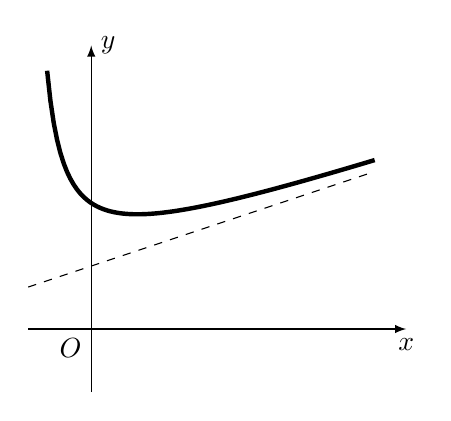
\begin{tikzpicture}[>=latex, scale=0.8]
    % Vẽ hệ trục
    \draw[->] (-1,0) -- (5,0) node[below] {$x$};
    \draw[->] (0,-1) -- (0,4.5) node[right] {$y$};
    \node[below left] at (0,0) {$O$};
    
    % Vẽ đồ thị hàm số
    \draw[ultra thick, samples=100, domain=-0.7:4.5] 
        plot (\x, {1/3*\x + 1 + 1/(\x + 1)});
    \draw[dashed, samples=100, domain=-1:4.5] 
        plot (\x, {1/3*\x + 1 });
    
\end{tikzpicture}
\end{center}}





% --- CÂU 2 ---
\questionTrueFalse{15}{6}{Lượng nước tưới cho vườn cây vào ngày thứ \( t \) (\( 1 \leq t \leq 30 \)) được ghi lại ở bảng sau. Biết rằng hàm số mô tả lượng nước tưới có dạng hàm số bậc ba.  
\begin{table}[h!]
\centering
\renewcommand{\arraystretch}{1.5} % Tăng khoảng cách dòng cho thoáng và giống ảnh mẫu
\begin{tabular}{|c|c|c|c|c|}
\hline
$t$ (ngày) & 2 & 6 & 12 & 18 \\ \hline
Lượng nước (lít) & 31 & 47 & 1571 & 7199 \\ \hline
\end{tabular}
\end{table}

}{
    \textbf{a)} & Hàm số mô tả lượng nước tưới vào ngày thứ \( t \) là \( y = 2t^3 - 15t^2 + 20t + 15 \).
    & \textcolor{amberorange}{$\bigcirc$} & \textcolor{amberorange}{$\bigcirc$} \\ \hline
    
    \textbf{b)} & Tại thời điểm ngày thứ 10, lượng nước đã tưới cho vườn cây là 320 lít.
    & \textcolor{amberorange}{$\bigcirc$} & \textcolor{amberorange}{$\bigcirc$} \\ \hline
    
    \textbf{c)} & Tâm đối xứng của đồ thị hàm số mô tả lượng nước tưới có tổng tung độ và hoành độ là 20.
    & \textcolor{amberorange}{$\bigcirc$} & \textcolor{amberorange}{$\bigcirc$} \\ \hline
    
    \textbf{d)} & Kể từ ngày thứ 10, lượng nước tưới đã vượt mức 700 lít.
    & \textcolor{amberorange}{$\bigcirc$} & \textcolor{amberorange}{$\bigcirc$} \\
}


% --- CÂU 4 ---
\questionTrueFalse{12}{7}{Tại công viên trung tâm, người ta xây một cầu vòm cong bằng thép bắc ngang qua một hồ nước nhỏ. Phần mép cong phía dưới của vòm cầu được thiết kế mô phỏng theo một phần của đồ thị hàm phân thức  
\(y = \dfrac{ax^2 + bx + c}{mx + n} \quad (a \neq 0, m \neq 0)\)
nhận \(x = -1\) là đường tiệm cận đứng. Đơn vị trên hệ trục tọa độ là mét.
\begin{center}
    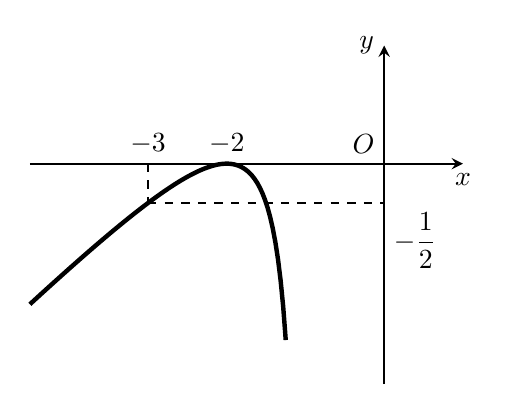
\begin{tikzpicture}[>=stealth, scale=1]

    % =================================================================
    % 1. VẼ HỆ TRỤC TỌA ĐỘ Oxy
    % =================================================================
    \draw[->, thick] (-4.5, 0) -- (1.0, 0) node[below] {$x$};
    \draw[->, thick] (0, -2.8) -- (0, 1.5) node[left] {$y$};
    
    % Gốc tọa độ O
    \node[above left] at (0,0) {$O$};

    % =================================================================
    % 2. VẼ ĐƯỜNG CONG ĐỒ THỊ (HÀM GHÉP ĐỂ ĐẠT ĐỘ DỐC NHƯ HÌNH VẼ)
    % =================================================================
    % Nhánh trái: parabol y = -0.5*(x+2)^2 đi qua (-3, -0.5) và đạt cực đại tại (-2, 0)
    \draw[ultra thick, samples=100, domain=-4.5:-1.25] plot (\x, {(\x*\x + 4*\x +4) /(\x+1)});
    
    

    % =================================================================
    % 3. VẼ CÁC ĐƯỜNG NÉT ĐỨT GIÓNG TỌA ĐỘ
    % =================================================================
    \draw[dashed, thick] (-3, 0) -- (-3, -0.5);
    \draw[dashed, thick] (-3, -0.5) -- (0, -0.5);

    % =================================================================
    % 4. GÁN NHÃN CÁC ĐIỂM TRÊN TRỤC TỌA ĐỘ
    % =================================================================
    \node[above] at (-3, 0) {$-3$};
    \node[above] at (-2, 0) {$-2$};
    \node[below right] at (0, -0.5) {$-\dfrac{1}{2}$};

\end{tikzpicture}
\end{center}
}{
    \textbf{a)} & Hàm số mô phỏng hình dạng vòm cầu là  
    \(f(x) = \dfrac{2(x + 2)^2}{x + 1}.\)
    & \textcolor{amberorange}{$\bigcirc$} & \textcolor{amberorange}{$\bigcirc$} \\ \hline
    
    \textbf{b)} & Điểm có tọa độ \(\left(-5; -\dfrac{9}{4}\right)\) thuộc đồ thị đường cong vòm cầu.
    & \textcolor{amberorange}{$\bigcirc$} & \textcolor{amberorange}{$\bigcirc$} \\ \hline
    
    \textbf{c)} & Đường tiệm cận xiên của đồ thị hàm số mô phỏng hình dạng vòm cầu là \(y = x + 3\).
    & \textcolor{amberorange}{$\bigcirc$} & \textcolor{amberorange}{$\bigcirc$} \\ \hline
    
    \textbf{d)} & Tại vị trí nằm trên vòm cầu cách trục \(Oy\) theo phương ngang một đoạn 4 mét thì điểm đó cách trục hoành một đoạn là \(\dfrac{8}{3}\) mét.
    & \textcolor{amberorange}{$\bigcirc$} & \textcolor{amberorange}{$\bigcirc$} \\
}






\end{document}
